\chapter{Appendix B. Parameter cross-sections from abundance matching MCMC.}

\label{Appx:AbnMCMC}
\lhead{Appendix B. \emph{Abundance Matching parameter cross-sections}}

Figure \ref{fig:MCMC_lz} shows the redshift $z = 0.1$ output from the MCMC abundance matching fits. It becomes immediately obvious that the low mass slope ($\beta$) is poorly constrained however the impact on the SMF is limited within the margin of error. The position of the knee (M) is well constrained against both the normalisation (N) and the high mass slope ($\gamma$). The shape of the constraint between the normalisation and gamma emanates from the need to produce high mass galaxies, if the normalisation is decreased the slope must increase to ensure enough haloes produce massive galaxies.

\begin{figure*}
	\centering
	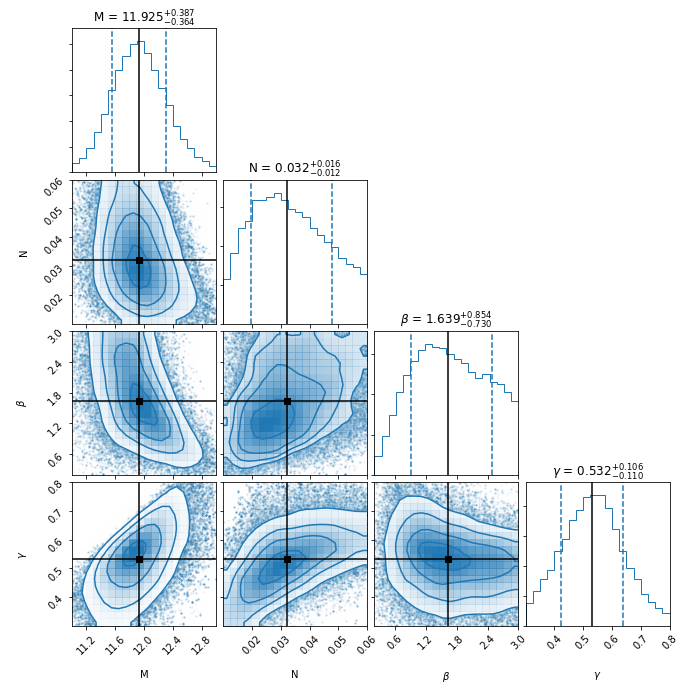
\includegraphics[width = \linewidth]{Appendices/AbnMCMC/MCMC_plot_lz.png}
    \caption{We show the MCMC parameter space for the redshift $z = 0.1$ fit. The position of the knee (M), the normalisation (N) the low mass slope ($\beta$) and the high mass slope ($\gamma$) are shown from left to right. Columns are titled with the best fit values and 16th/84th percentile errors. The black lines show the best fit value with a black square at intersections, the 16th/84th percentiles are shown with blue dashed lines on the histograms.}
	\label{fig:MCMC_lz}
\end{figure*}

Figure \ref{fig:MCMC_hz} shows the redshift $z > 0.1$ output from the MCMC abundance matching fits. All parameters have low evolution and the SMHM relation evolves only weakly with redshift. For M, $\beta$, and $\gamma$ where the distributions are wide  or close to the prior we have tested wider priors and insignificant change is found.

\begin{figure*}
	\centering
	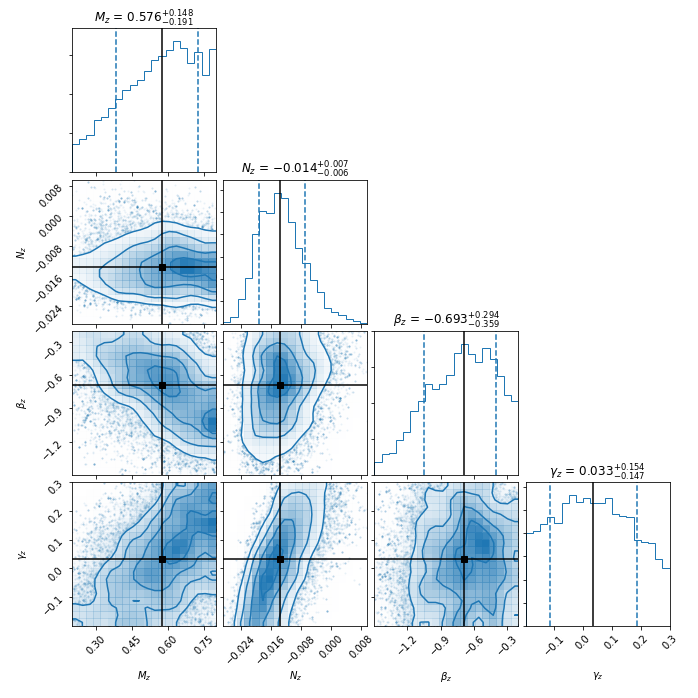
\includegraphics[width = \linewidth]{Appendices/AbnMCMC/MCMC_plot_hz.png}
    \caption{We show the MCMC parameter space for the high redshift $z > 0.1$ fit. The evolution of: the position of the knee ($M_z$), the normalisation ($N_z$) the low mass slope ($\beta_z$) and the high mass slope ($\gamma_z$) are shown from left to right. Columns are titled with the best fit values and 16th/84th percentile errors. The black lines show the best fit value with a black square at intersections, the 16th/84th percentiles are shown with blue dashed lines on the histograms.}
	\label{fig:MCMC_hz}
\end{figure*}